\documentclass{article}
\usepackage[hyphens]{url}
\usepackage{mathtools}
\usepackage{amsmath}
\usepackage{listings}
\usepackage{graphicx}
\usepackage[margin=1in]{geometry}
\usepackage{float}
\floatstyle{boxed}
\restylefloat{figure}
\lstset{basicstyle=\footnotesize, breaklines=true}
\begin{document}


\title{CS595 Intro to Web Science, Assignment \#9}
\author{Valentina Neblitt-Jones}
\date{December 5, 2013}
\maketitle

\newpage
\listoftables
\lstlistoflistings
\listoffigures

\newpage
\section*{Question 1}

Create a blog-term matrix. Start by grabbing 100 blogs; include: \\

\begin{itemize}
\item \url{http://f-measure.blogspot.com/}
\item \url{http://ws-dl.blogspot.com/}
\end{itemize}

and grab 98 more as per the method shown in class. \\

Use the blog title as the identifier for each blog (and row of the matrix). Use the terms from every item/title (RSS) or entry/title (Atom) for the columns of the matrix. The values are the frequency of occurrence. Essentially you are replicating the format of the ``blogdata.txt'' file included with the PCI book code. Limit the number of terms to the most ``popular'' (i.e., frequent) 500 terms, this is \textbf{after} the criteria on p. 32 (slide 7) has been satisfied.

\subsection*{Answer to Question 1}
For this question, I had to use three scripts (1) getFeedList.py, (2) generatefeedvector.py and (3) reduceTerms.py. 
\begin{figure}[H]
\centering
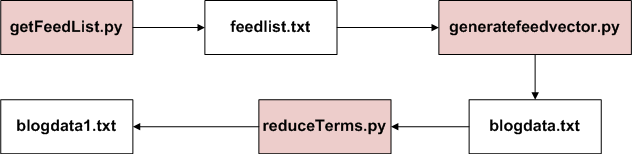
\includegraphics[scale=0.50]{q01/FlowForQ1}
\caption{Creation of the Blog-Term Matrix}
\label{FlowForQ1}
\end{figure}

In Listing \ref{getFeedList} (getFeedList.py), I ``manually'' added F-Measure and the WS-DL blogs, but creating the empty list feedlist and added those two blogs first. I then used the link for next blog \url{http://www.blogger.com/next-blog?navBar=true&blogID=3471633091411211117} in a while loop to create a list of random blogs. I capture the atom feed uri using BeautifulSoup. I had to include the sleep function since my script stopped running before reaching even 10 blogs. I added the ``?max-results=200'' to each uri so that it would grab at most 200 entries. This script produced feedlist.txt as an output.

I used generatefeedvector.py (Listing \ref{generatefeedvector}) from the book \cite{pci}. I had to make minimal changes to it in order to handle an encoding error I had encountered. Some blog titles had special characters like the copyright symbol and there was one blog with a title written in Chinese. This script accepted feedlist.txt as an input and produced blogdata.txt as an output. My term output was approximately 3200 terms.

The final part of the problem was to take the 3200+ terms and reduce it to the 500 most frequent terms. In listing \ref{reduceTerms} (reduceTerms.py), 
I imported clusters.py in order to read in the blogdata.txt file. I then created an empty dictionary to store the sums of the term occurrences. I looped through the words which served as columns and summed the frequency. I then reverse sorted the dictionary and limited to the first 500 terms. Next I eliminate all the other terms from the matrix by only including terms that were found in the reverse sorted limited collection.

\newpage
\section*{Question 2}
Create an ASCII and JPEG dendrogram that clusters (i.e., HAC) the most similar blogs (see slides 12 \& 13). Include the JPEG in your report and upload the ASCII file to GitHub (it will be too unwieldy for inclusion in the report.)

\subsection*{Answer to Question 2}

To answer this question, I relied on clusters.py and used the code samples from page 37 and page 40 of the book \cite{pci} and included them generateImages.py (Listing \ref{generateImages}). The ASCII dendrogram is located in GitHub at \url{https://github.com/vneblitt/cs595-f13/blob/master/assignment09/q02/blogclustascii.txt}. The JPEG dendrogram using Python Imaging Library (PIL) is Figure \ref{blogclust}.

\begin{lstlisting}[frame=single, caption=generateImages.py, label=generateImages]
import sys

sys.path.insert(0, '/Users/vneblitt/Documents/cs595-f13/assignment09/library')

import clusters

# Create clusters
blognames,words,data=clusters.readfile('/Users/vneblitt/Documents/cs595-f13/assignment09/q01/blogdata1.txt')
clust=clusters.hcluster(data)

# Create ASCII dendrogram
clusters.printclust(clust,labels=blognames)

# Create Nicer dendrogram with PIL
clusters.drawdendrogram(clust,blognames,jpeg='blogclust.jpg')
\end{lstlisting}

It is quite difficult to see Figure \ref{blogclust}, but a selected close-up (see Figure \ref{musicblogs}) shows that some of the clustering was moderately successful. 

\begin{figure}[H]
\centering
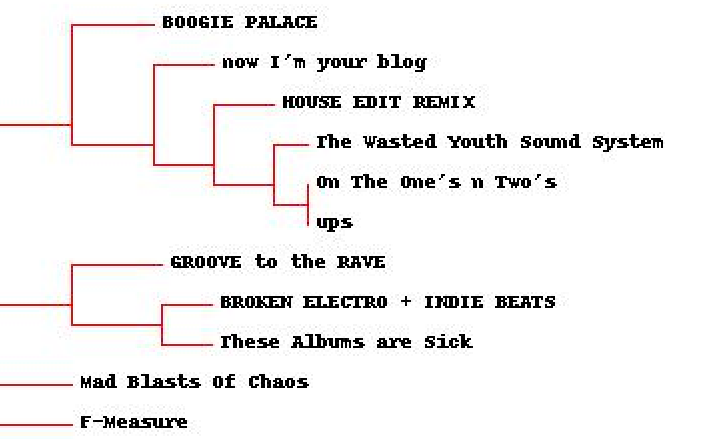
\includegraphics[scale=0.50]{q02/musicblogs}
\caption{Music Blogs in Dendrogram}
\label{musicblogs}
\end{figure}

\begin{figure}[H]
\centering
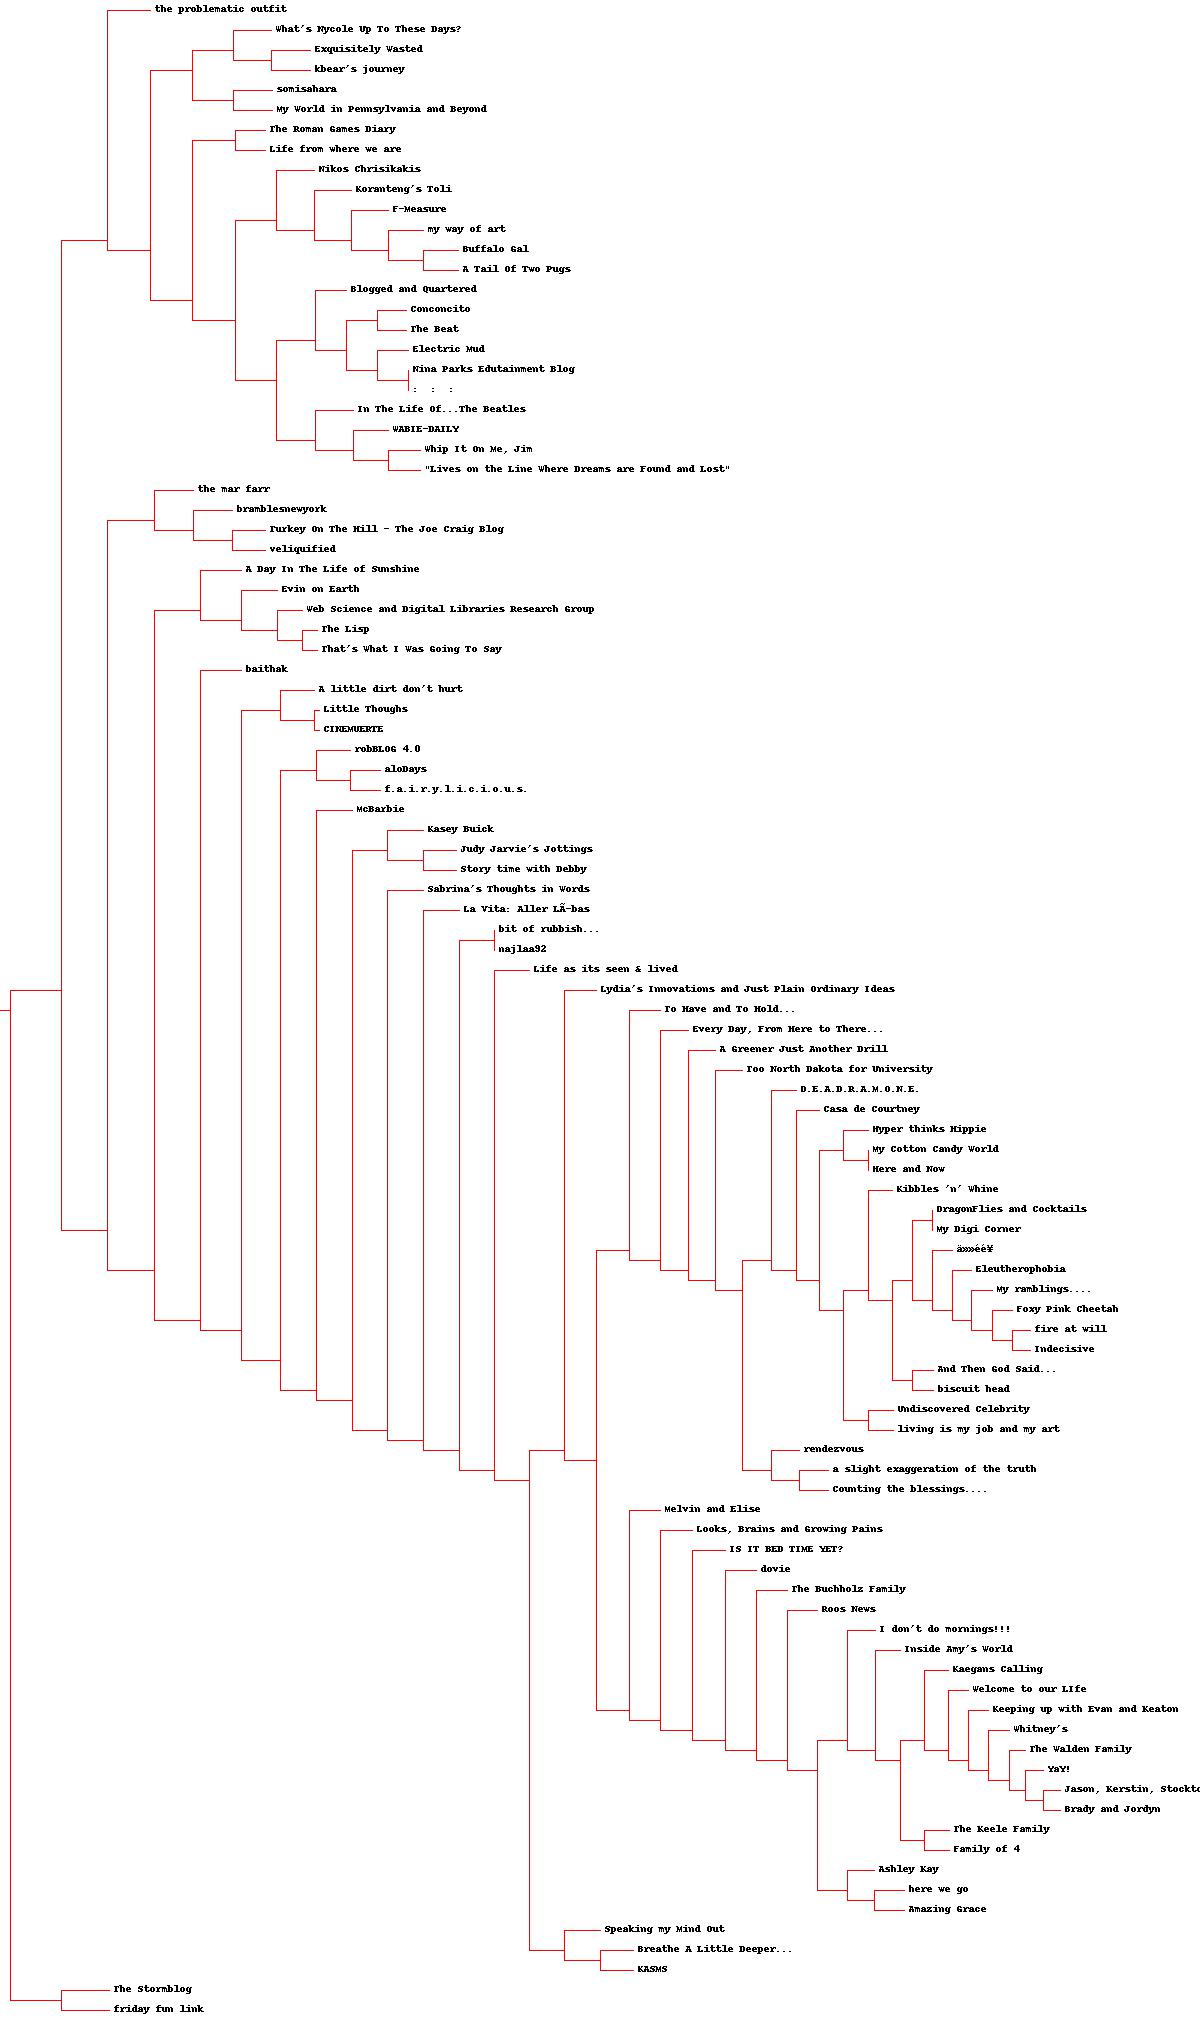
\includegraphics[scale=0.30]{q02/blogclust}
\caption{JPEG Dendrogram}
\label{blogclust}
\end{figure}



\newpage
\section*{Question 3}
Cluster the blogs using K-Means, using k=5, 10, 20 (see slide 18). How many iterations were required for each value of k?

\subsection*{Answer to Question 3}

To answer this question, I again relied on clusters.py and used the code samples from page 44 of the book \cite{pci} and included them getKMeans.py (Listing \ref{getKMeans}). I ran this a few times and got different results each time. Segaran explains this in Chapter 3, ``Because this function uses random centroids to start with, the order of the results retired will almost always be different. It's also possible for the contents of the clusters to be different depending on the initial locations of the centroids.''\cite{pci} Listing \ref{kmeansoutput} shows the actual output of the script and Table 1 shows the summary data.

\begin{lstlisting}[frame=single, caption=getKMeans.py, label=getKMeans]
import sys

sys.path.insert(0, '/Users/vneblitt/Documents/cs595-f13/assignment09/library')

import clusters

blognames,words,data=clusters.readfile('/Users/vneblitt/Documents/cs595-f13/assignment09/q01/blogdata1.txt')

print 'k=5'
kclust=clusters.kcluster(data,k=5)

print 'k=10'
kclust=clusters.kcluster(data,k=10)

print 'k=20'
kclust=clusters.kcluster(data,k=20)
\end{lstlisting}

\begin{table}[!h]
\centering
\begin{tabular}{c c}
Value of k & No. of Iterations \\
\hline
5 & 6  \\
10 & 7  \\
20 & 100  \\
\hline
\end{tabular}
\caption{K-Means Iterations}
\end{table}

\newpage
\section*{Question 4}
Use MDS to create a JPG of the blogs similar to slide 29. How many iterations were required?

\subsection*{Answer to Question 4}

I had to reduce the MDS image down to 20\% in order to include it in this report, but that makes it too hard to read (see Figure \ref{blogs2d}). The full one is located in GitHub at \url{https://github.com/vneblitt/cs595-f13/blob/master/assignment09/q04/blogs2d.jpg}.

When I first ran the code, I encounter a divide-by-zero error that would not allow the code to fully execute. I had to remove the following four blogs from the blog-term matrix since their entire row in the matrix contained zeros.

\begin{itemize}
\item Blonde Ambition
\item ups
\item Alcorn Studios
\item All Scattered
\end{itemize}

I ran into this problem earlier when I had only managed to get 60 terms from Q1. I thought I would not encounter this problem since I included the summaries and descriptions had achieved 3200+ terms and then reduced the terms down to the 500 most frequent.

\begin{lstlisting}[frame=single, caption=getMDS.py, label=getMDS]
import sys

sys.path.insert(0, '/Users/vneblitt/Documents/cs595-f13/assignment09/library')

import clusters

blognames,words,data=clusters.readfile('blogdata1.txt')

coords=clusters.scaledown(data)
clusters.draw2d(coords,blognames,jpeg='blogs2d.jpg')
\end{lstlisting}

I examined blogs listed near F-Measure in the close-up (Figure \ref{musicMDS}) and saw most of the same ones in the JPEG dendrogram. P-Money was a new one. The MDS took 177 iterations (Listing \ref{MDSoutput}).

\begin{figure}[H]
\centering
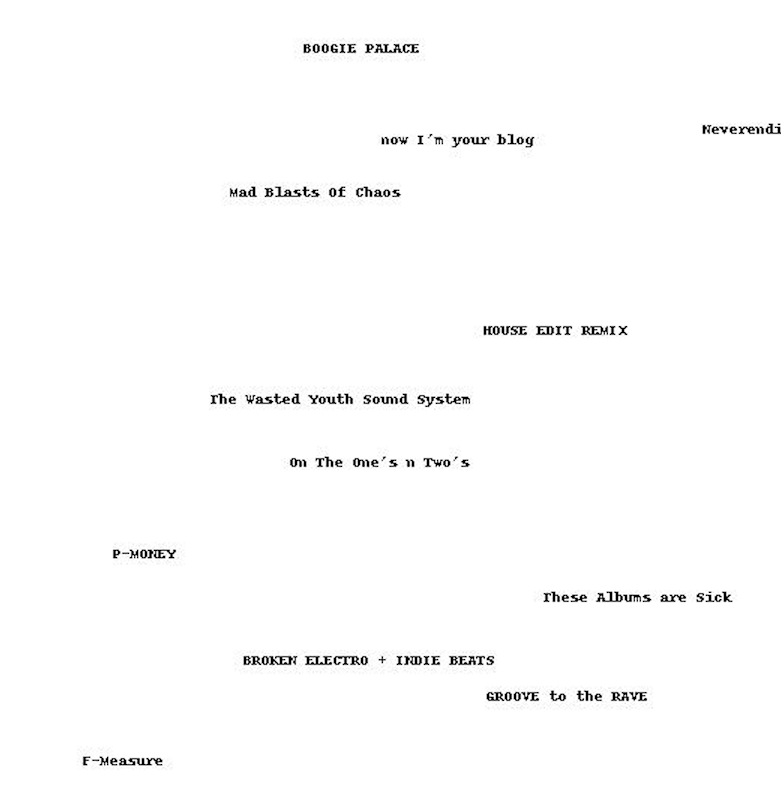
\includegraphics[scale=0.50]{q04/musicMDS}
\caption{Music Blogs with MDS}
\label{musicMDS}
\end{figure}

\begin{figure}[H]
\centering
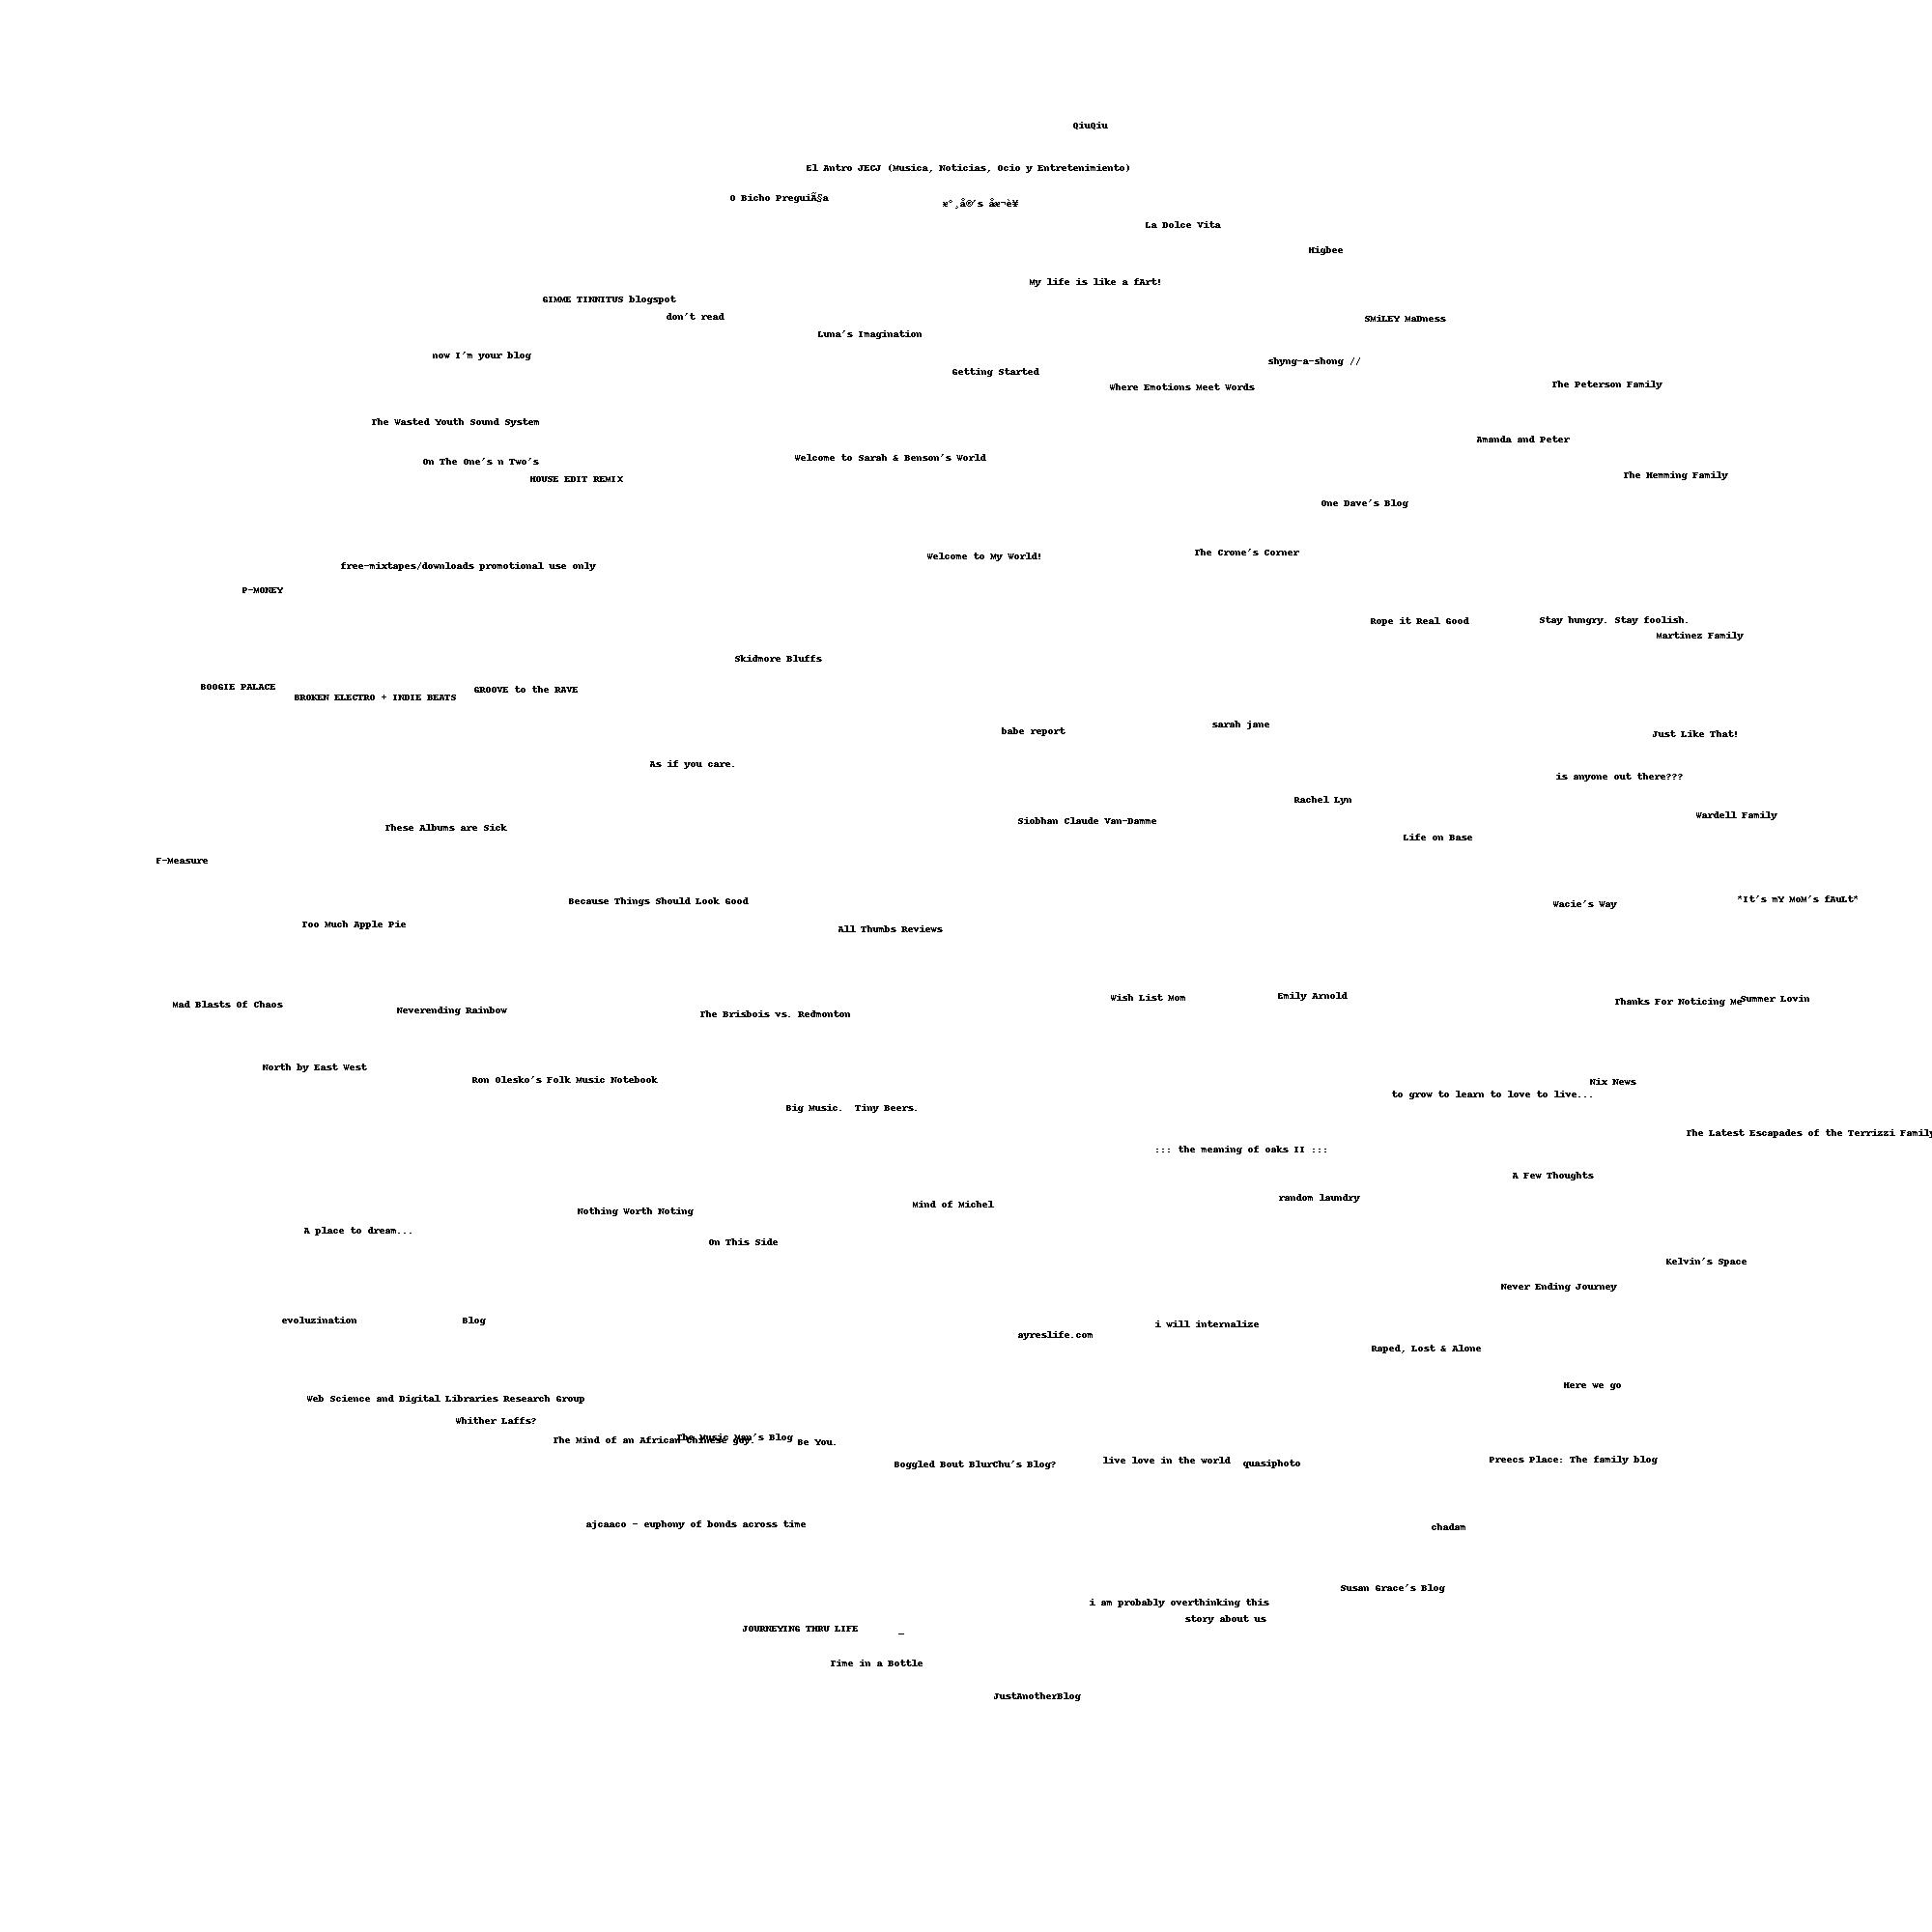
\includegraphics[scale=0.20]{q04/blogs2d}
\caption{Multi-Dimenional Scaling}
\label{blogs2d}
\end{figure}

\newpage

\section*{Question 5 - Extra Credit (5 points)}
Re-run Q2, but this time with proper TFIDF calculations instead of the hack discussed on slide 7 (p. 32). Use the same 500 words, but this time replace their frequency count with TFIDF scores as computed in assignment \#3. Document the code, techniques, methods, etc. used to generate these TFIDF values. Upload the new file to GitHub. \\

Compare and contrast the resulting dendrogram with the dendrogram from Q2. \\

Note: Ideally you would not reuse the same 500 terms and instead come up with TFIDF scores for all the terms and choose the top 500 from that list, but I am trying to limit the amount of work necessary.

\subsection*{Answer to Question 5}

Not attempted.

%\renewcommand\thesubsection{\arabic{subsection}}
%\subsection{What 5 movies have the highest average ratings? Show the movies and their ratings sorted by their average ratings.}

%\begin{lstlisting}[frame=single, caption=highestavgrating.py, label=highaverage]
%\end{lstlisting}

%\newpage
%\subsection{What 5 movies have received the most ratings? Show the movies and the number of ratings sorted by number of ratings.}

%\begin{table}[!h]
%\centering
%\begin{tabular}{l c}
%Movie Title & No. of Ratings \\
%\hline
%Star Wars (1977) & 583  \\
%Contact (1997) & 509  \\
%Fargo (1996) & 508  \\
%Return of the Jedi (1983) & 507  \\
%Marlene Dietrich: Shadow and Light (1997) & 485  \\
%\hline
%\end{tabular}
%\caption{Movies with the Most Ratings}
%\end{table}

%\begin{figure}[H]
%\centering
%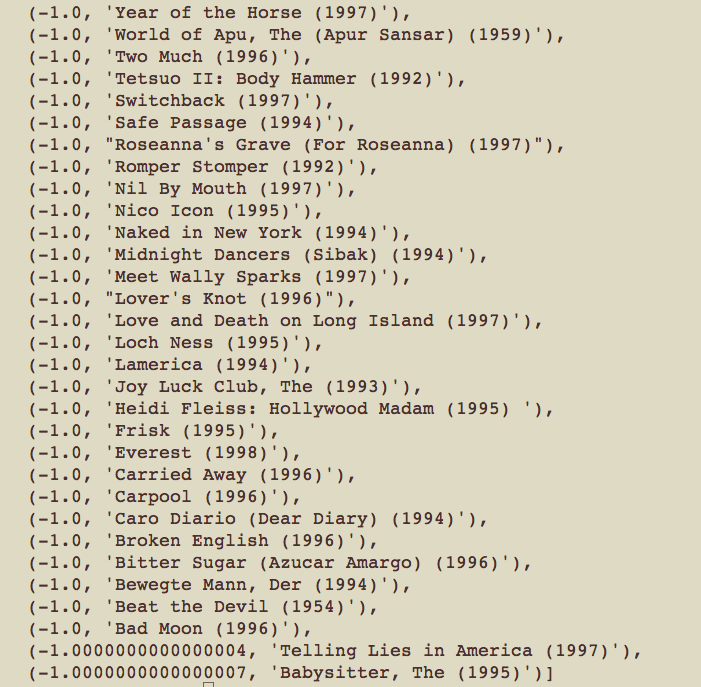
\includegraphics[scale=0.50]{q05/leastliketopgun}
%\caption{Movies Least Like Top Gun}
%\label{leastliketopgun}
%\end{figure}

\newpage
\appendix

\section{getFeedList.py}

\begin{lstlisting}[frame=single, caption=getFeedList.py, label=getFeedList]

from bs4 import BeautifulSoup
from urllib2 import HTTPError
import urllib2
import time

f = open('feedlist.txt', 'w')

# These two are automatically in the list
firstfeed = 'http://f-measure.blogspot.com/feeds/posts/default'
secondfeed = 'http://ws-dl.blogspot.com/feeds/posts/default'

feedlist = []
feedlist.append(firstfeed)
feedlist.append(secondfeed)

while len(feedlist) <= 100:
    try:

        nextblog = 'http://www.blogger.com/next-blog?navBar=true&blogID=3471633091411211117'

        html = urllib2.urlopen(nextblog).read()

        soup = BeautifulSoup(html)

        atomfeedurl = soup.find_all('link', attrs = {'type' : 'application/atom+xml'})[0].attrs['href']

    except HTTPError as h:
        pass

    except IndexError as i:
        pass

    if atomfeedurl:

        if atomfeedurl not in feedlist:

            print atomfeedurl
            feedlist.append(atomfeedurl)

    time.sleep(1)

for item in feedlist:
    f.write(item + '?max-results=200' + '\n')

f.close()

\end{lstlisting}

\section{generatefeedvector.py}

\begin{lstlisting}[frame=single, caption=generatefeedvector.py, label=generatefeedvector]
import feedparser
import re

# Returns title and dictionary of word counts for an RSS feed
def getwordcounts(url):
  # Parse the feed
  d=feedparser.parse(url)
  wc={}

  # Loop over all the entries
  for e in d.entries:
      if 'summary' in e: summary=e.summary
      else: summary=e.description

    # Extract a list of words
      words=getwords(e.title+' '+summary)
      for word in words:
        wc.setdefault(word,0)
        wc[word]+=1
  return d.feed.title,wc

def getwords(html):
  # Remove all the HTML tags
  txt=re.compile(r'<[^>]+>').sub('',html)

  # Split words by all non-alpha characters
  words=re.compile(r'[^A-Z^a-z]+').split(txt)

  # Convert to lowercase
  return [word.lower() for word in words if word!='']


apcount={}
wordcounts={}
feedlist=[line for line in file('feedlist.txt')]
for feedurl in feedlist:
  try:
    title,wc=getwordcounts(feedurl)
    wordcounts[title]=wc
    for word,count in wc.items():
      apcount.setdefault(word,0)
      if count>1:
        apcount[word]+=1
  except:
    print 'Failed to parse feed %s' % feedurl

wordlist=[]
for w,bc in apcount.items():
  frac=float(bc)/len(feedlist)
  if frac>0.1 and frac<0.5:
    wordlist.append(w)

out=file('blogdata.txt','w')
out.write('Blog')
for word in wordlist: out.write('\t%s' % word)
out.write('\n')
for blog,wc in wordcounts.items():
  print blog
  blog = blog.encode('UTF-8')
  out.write(blog)
  for word in wordlist:
    if word in wc: out.write('\t%d' % wc[word])
    else: out.write('\t0')
  out.write('\n')
\end{lstlisting}

\section{reduceTerms.py}

\begin{lstlisting}[frame=single, caption=reduceTerms.py, label=reduceTerms]
import sys

sys.path.insert(0, '/Users/vneblitt/Documents/cs595-f13/assignment09/library')

import clusters

blognames,words,data=clusters.readfile('blogdata.txt')

# row
# print 'blog name: ' + blognames[0]

# column
# print 'term: ' + words[3]

# junction
# print 'value: ' + str(data[0][3])

# print 'number of blogs: ' + str(len(blognames))
# print 'number of words: ' + str(len(words))

wordsums={}

for j in range(len(words)):
	sum = 0
	for i in range (len(blognames)):
		sum = sum + data[i][j]
	# print words[j] + ' ' + str(sum)
	wordsums[j] = int(sum)
	
# print wordsums

a = sorted(wordsums, key=wordsums.get, reverse=True)[0:500]

# print (len(a))

# print a

print 'Blog',

for m in range(len(words)):
	if m in a:
		print '\t' + words[m],
print

for i in range(len(blognames)):
	print blognames[i],
		
	for j in range(len(words)):
		if j in a:
			print '\t' + str(int(data[i][j])),
			
	print
\end{lstlisting}

\section{clusters.py}

This code is used for Q2, Q3, and Q4.

\begin{lstlisting}[frame=single, caption=clusters.py, label=clusters]
from PIL import Image,ImageDraw

def readfile(filename):
  lines=[line for line in file(filename)]
  
  # First line is the column titles
  colnames=lines[0].strip().split('\t')[1:]
  rownames=[]
  data=[]
  for line in lines[1:]:
    p=line.strip().split('\t')
    # First column in each row is the rowname
    rownames.append(p[0])
    # The data for this row is the remainder of the row
    data.append([float(x) for x in p[1:]])
  return rownames,colnames,data


from math import sqrt

def pearson(v1,v2):
  # Simple sums
  sum1=sum(v1)
  sum2=sum(v2)
  
  # Sums of the squares
  sum1Sq=sum([pow(v,2) for v in v1])
  sum2Sq=sum([pow(v,2) for v in v2])	
  
  # Sum of the products
  pSum=sum([v1[i]*v2[i] for i in range(len(v1))])
  
  # Calculate r (Pearson score)
  num=pSum-(sum1*sum2/len(v1))
  den=sqrt((sum1Sq-pow(sum1,2)/len(v1))*(sum2Sq-pow(sum2,2)/len(v1)))
  if den==0: return 0

  return 1.0-num/den

class bicluster:
  def __init__(self,vec,left=None,right=None,distance=0.0,id=None):
    self.left=left
    self.right=right
    self.vec=vec
    self.id=id
    self.distance=distance

def hcluster(rows,distance=pearson):
  distances={}
  currentclustid=-1

  # Clusters are initially just the rows
  clust=[bicluster(rows[i],id=i) for i in range(len(rows))]

  while len(clust)>1:
    lowestpair=(0,1)
    closest=distance(clust[0].vec,clust[1].vec)

    # loop through every pair looking for the smallest distance
    for i in range(len(clust)):
      for j in range(i+1,len(clust)):
        # distances is the cache of distance calculations
        if (clust[i].id,clust[j].id) not in distances: 
          distances[(clust[i].id,clust[j].id)]=distance(clust[i].vec,clust[j].vec)

        d=distances[(clust[i].id,clust[j].id)]

        if d<closest:
          closest=d
          lowestpair=(i,j)

    # calculate the average of the two clusters
    mergevec=[
    (clust[lowestpair[0]].vec[i]+clust[lowestpair[1]].vec[i])/2.0 
    for i in range(len(clust[0].vec))]

    # create the new cluster
    newcluster=bicluster(mergevec,left=clust[lowestpair[0]],
                         right=clust[lowestpair[1]],
                         distance=closest,id=currentclustid)

    # cluster ids that weren't in the original set are negative
    currentclustid-=1
    del clust[lowestpair[1]]
    del clust[lowestpair[0]]
    clust.append(newcluster)

  return clust[0]

def printclust(clust,labels=None,n=0):
  # indent to make a hierarchy layout
  for i in range(n): print ' ',
  if clust.id<0:
    # negative id means that this is branch
    print '-'
  else:
    # positive id means that this is an endpoint
    if labels==None: print clust.id
    else: print labels[clust.id]

  # now print the right and left branches
  if clust.left!=None: printclust(clust.left,labels=labels,n=n+1)
  if clust.right!=None: printclust(clust.right,labels=labels,n=n+1)

def getheight(clust):
  # Is this an endpoint? Then the height is just 1
  if clust.left==None and clust.right==None: return 1

  # Otherwise the height is the same of the heights of
  # each branch
  return getheight(clust.left)+getheight(clust.right)

def getdepth(clust):
  # The distance of an endpoint is 0.0
  if clust.left==None and clust.right==None: return 0

  # The distance of a branch is the greater of its two sides
  # plus its own distance
  return max(getdepth(clust.left),getdepth(clust.right))+clust.distance


def drawdendrogram(clust,labels,jpeg='clusters.jpg'):
  # height and width
  h=getheight(clust)*20
  w=1200
  depth=getdepth(clust)

  # width is fixed, so scale distances accordingly
  scaling=float(w-150)/depth

  # Create a new image with a white background
  img=Image.new('RGB',(w,h),(255,255,255))
  draw=ImageDraw.Draw(img)

  draw.line((0,h/2,10,h/2),fill=(255,0,0))    

  # Draw the first node
  drawnode(draw,clust,10,(h/2),scaling,labels)
  img.save(jpeg,'JPEG')

def drawnode(draw,clust,x,y,scaling,labels):
  if clust.id<0:
    h1=getheight(clust.left)*20
    h2=getheight(clust.right)*20
    top=y-(h1+h2)/2
    bottom=y+(h1+h2)/2
    # Line length
    ll=clust.distance*scaling
    # Vertical line from this cluster to children    
    draw.line((x,top+h1/2,x,bottom-h2/2),fill=(255,0,0))    
    
    # Horizontal line to left item
    draw.line((x,top+h1/2,x+ll,top+h1/2),fill=(255,0,0))    

    # Horizontal line to right item
    draw.line((x,bottom-h2/2,x+ll,bottom-h2/2),fill=(255,0,0))        

    # Call the function to draw the left and right nodes    
    drawnode(draw,clust.left,x+ll,top+h1/2,scaling,labels)
    drawnode(draw,clust.right,x+ll,bottom-h2/2,scaling,labels)
  else:   
    # If this is an endpoint, draw the item label
    draw.text((x+5,y-7),labels[clust.id],(0,0,0))

def rotatematrix(data):
  newdata=[]
  for i in range(len(data[0])):
    newrow=[data[j][i] for j in range(len(data))]
    newdata.append(newrow)
  return newdata

import random

def kcluster(rows,distance=pearson,k=4):
  # Determine the minimum and maximum values for each point
  ranges=[(min([row[i] for row in rows]),max([row[i] for row in rows])) 
  for i in range(len(rows[0]))]

  # Create k randomly placed centroids
  clusters=[[random.random()*(ranges[i][1]-ranges[i][0])+ranges[i][0] 
  for i in range(len(rows[0]))] for j in range(k)]
  
  lastmatches=None
  for t in range(100):
    print 'Iteration %d' % t
    bestmatches=[[] for i in range(k)]
    
    # Find which centroid is the closest for each row
    for j in range(len(rows)):
      row=rows[j]
      bestmatch=0
      for i in range(k):
        d=distance(clusters[i],row)
        if d<distance(clusters[bestmatch],row): bestmatch=i
      bestmatches[bestmatch].append(j)

    # If the results are the same as last time, this is complete
    if bestmatches==lastmatches: break
    lastmatches=bestmatches
    
    # Move the centroids to the average of their members
    for i in range(k):
      avgs=[0.0]*len(rows[0])
      if len(bestmatches[i])>0:
        for rowid in bestmatches[i]:
          for m in range(len(rows[rowid])):
            avgs[m]+=rows[rowid][m]
        for j in range(len(avgs)):
          avgs[j]/=len(bestmatches[i])
        clusters[i]=avgs
      
  return bestmatches

def tanamoto(v1,v2):
  c1,c2,shr=0,0,0
  
  for i in range(len(v1)):
    if v1[i]!=0: c1+=1 # in v1
    if v2[i]!=0: c2+=1 # in v2
    if v1[i]!=0 and v2[i]!=0: shr+=1 # in both
  
  return 1.0-(float(shr)/(c1+c2-shr))

def scaledown(data,distance=pearson,rate=0.01):
  n=len(data)

  # The real distances between every pair of items
  realdist=[[distance(data[i],data[j]) for j in range(n)] 
             for i in range(0,n)]

  # Randomly initialize the starting points of the locations in 2D
  loc=[[random.random(),random.random()] for i in range(n)]
  fakedist=[[0.0 for j in range(n)] for i in range(n)]
  
  lasterror=None
  for m in range(0,1000):
    # Find projected distances
    for i in range(n):
      for j in range(n):
        fakedist[i][j]=sqrt(sum([pow(loc[i][x]-loc[j][x],2) 
                                 for x in range(len(loc[i]))]))
  
    # Move points
    grad=[[0.0,0.0] for i in range(n)]
    
    totalerror=0
    for k in range(n):
      for j in range(n):
        if j==k: continue
        # The error is percent difference between the distances
        errorterm=(fakedist[j][k]-realdist[j][k])/realdist[j][k]
        
        # Each point needs to be moved away from or towards the other
        # point in proportion to how much error it has
        grad[k][0]+=((loc[k][0]-loc[j][0])/fakedist[j][k])*errorterm
        grad[k][1]+=((loc[k][1]-loc[j][1])/fakedist[j][k])*errorterm

        # Keep track of the total error
        totalerror+=abs(errorterm)
    print totalerror

    # If the answer got worse by moving the points, we are done
    if lasterror and lasterror<totalerror: break
    lasterror=totalerror
    
    # Move each of the points by the learning rate times the gradient
    for k in range(n):
      loc[k][0]-=rate*grad[k][0]
      loc[k][1]-=rate*grad[k][1]

  return loc

def draw2d(data,labels,jpeg='mds2d.jpg'):
  img=Image.new('RGB',(2000,2000),(255,255,255))
  draw=ImageDraw.Draw(img)
  for i in range(len(data)):
    x=(data[i][0]+0.5)*1000
    y=(data[i][1]+0.5)*1000
    draw.text((x,y),labels[i],(0,0,0))
  img.save(jpeg,'JPEG') 
\end{lstlisting}

\section{Output from getKMeans.py}

\begin{lstlisting}[frame=single, caption=kmeansoutput.txt, label=kmeansoutput]
k=5
Iteration 0
Iteration 1
Iteration 2
Iteration 3
Iteration 4
Iteration 5
k=10
Iteration 0
Iteration 1
Iteration 2
Iteration 3
Iteration 4
Iteration 5
Iteration 6
k=20
Iteration 0
Iteration 1
Iteration 2
Iteration 3
Iteration 4
Iteration 5
Iteration 6
Iteration 7
Iteration 8
Iteration 9
Iteration 10
Iteration 11
Iteration 12
Iteration 13
Iteration 14
Iteration 15
Iteration 16
Iteration 17
Iteration 18
Iteration 19
Iteration 20
Iteration 21
Iteration 22
Iteration 23
Iteration 24
Iteration 25
Iteration 26
Iteration 27
Iteration 28
Iteration 29
Iteration 30
Iteration 31
Iteration 32
Iteration 33
Iteration 34
Iteration 35
Iteration 36
Iteration 37
Iteration 38
Iteration 39
Iteration 40
Iteration 41
Iteration 42
Iteration 43
Iteration 44
Iteration 45
Iteration 46
Iteration 47
Iteration 48
Iteration 49
Iteration 50
Iteration 51
Iteration 52
Iteration 53
Iteration 54
Iteration 55
Iteration 56
Iteration 57
Iteration 58
Iteration 59
Iteration 60
Iteration 61
Iteration 62
Iteration 63
Iteration 64
Iteration 65
Iteration 66
Iteration 67
Iteration 68
Iteration 69
Iteration 70
Iteration 71
Iteration 72
Iteration 73
Iteration 74
Iteration 75
Iteration 76
Iteration 77
Iteration 78
Iteration 79
Iteration 80
Iteration 81
Iteration 82
Iteration 83
Iteration 84
Iteration 85
Iteration 86
Iteration 87
Iteration 88
Iteration 89
Iteration 90
Iteration 91
Iteration 92
Iteration 93
Iteration 94
Iteration 95
Iteration 96
Iteration 97
Iteration 98
Iteration 99
\end{lstlisting}

\section{Output from getMDS.py}

\begin{lstlisting}[frame=single, caption=MDSoutput.txt, label=MDSoutput]
4303.48133321
3263.8719182
3229.08048926
3213.98144395
3205.42081727
3198.88211785
3193.3356909
3187.77342166
3183.3231479
3179.40667134
3175.22192384
3170.96960085
3166.96684257
3163.62276825
3160.56855218
3158.19659115
3155.76372143
3153.26828583
3150.5325113
3147.91489254
3145.35701557
3143.14598618
3141.1417931
3139.17432119
3137.07921751
3135.07605846
3133.20975681
3131.44888509
3129.43360402
3127.56953291
3125.71742972
3123.74010891
3121.64718565
3119.52399267
3117.32009215
3115.08579695
3112.48797983
3109.92562616
3107.47776269
3104.91067682
3102.4132777
3100.1425645
3097.86818486
3095.52047081
3093.19536232
3090.81342075
3088.24281394
3085.46256414
3082.4847589
3079.59424177
3076.24654797
3072.80617316
3069.05803098
3065.2499318
3062.08903586
3058.99554788
3055.93645095
3052.33362152
3048.77735069
3045.58887204
3042.1009157
3038.91053247
3036.1025499
3033.23462166
3030.01657225
3026.68130791
3023.3538693
3020.07480977
3016.85469822
3013.67243951
3010.84137323
3008.21244992
3005.64359536
3003.48349187
3001.37717612
2999.3523348
2997.68075277
2995.95737554
2994.18375677
2992.20897228
2990.35136582
2988.61789689
2986.95074538
2985.34421086
2983.81342635
2982.43393729
2981.08756679
2979.65893465
2978.28724285
2976.92891057
2975.42200734
2973.8024168
2972.26218378
2970.76691141
2969.21264155
2967.43755513
2965.61122354
2963.65379455
2961.78272151
2960.33339597
2958.99112838
2957.61339024
2956.2869599
2955.1847749
2954.19000499
2953.21354625
2952.15353013
2950.93640415
2949.82195712
2948.77665761
2947.9995648
2947.27419277
2946.63124613
2945.89654206
2945.21428297
2944.39980467
2943.36331896
2942.35265457
2941.35613863
2940.46244284
2939.66125461
2938.84023767
2937.92341992
2937.01553795
2936.16134311
2935.39602156
2934.76968578
2934.04277107
2933.31445777
2932.5954256
2931.78290188
2930.88014992
2929.94347925
2929.16075115
2928.53948347
2927.97822488
2927.51401586
2927.05985204
2926.56553965
2926.07524921
2925.61746815
2925.32387562
2925.09225605
2924.85919982
2924.59414414
2924.36902247
2924.14572214
2923.88588256
2923.6019601
2923.36306561
2923.25188994
2923.12576899
2922.9102469
2922.6242511
2922.35262929
2922.09895422
2921.94417344
2921.84972487
2921.7352673
2921.61015403
2921.46562313
2921.24943948
2921.03583087
2920.78589764
2920.68330467
2920.65963508
2920.60454956
2920.56112372
2920.54432748
2920.52590698
2920.49261074
2920.44941975
2920.41992387
2920.36934944
2920.3172678
2920.26764289
2920.28033497
\end{lstlisting}

\newpage

\bibliographystyle{acm}
\bibliography{references}

\end{document}